
%%%%%%%%%%%%%%%%%%%%%%% file typeinst.tex %%%%%%%%%%%%%%%%%%%%%%%%%
%
% This is the LaTeX source for the TDPTemplate using
% the LaTeX document class 'llncs.cls' Springer LNAI format
% used in the RoboCup Symposium submissions.
% http://www.springer.com/computer/lncs?SGWID=0-164-6-793341-0
%
% It may be used as a template for your own TDP - copy it
% to a new file with a new name and use it as the basis
% for your Team Description Paper
%
% NB: the document class 'llncs' has its own and detailed documentation, see
% ftp://ftp.springer.de/data/pubftp/pub/tex/latex/llncs/latex2e/llncsdoc.pdf
%
%%%%%%%%%%%%%%%%%%%%%%%%%%%%%%%%%%%%%%%%%%%%%%%%%%%%%%%%%%%%%%%%%%%

\documentclass[runningheads,a4paper]{llncs}

% document input
\usepackage[utf8]{inputenc}		% input encoding
\usepackage[english]{babel}		% input language for hyphens

% fonts 
\usepackage[T1]{fontenc}		% more glyphs and a
\usepackage{lmodern}			% better looking font

% page geometry
%\usepackage{a4wide}
%\usepackage{a4}
%\usepackage[left=48mm,right=46mm]{geometry}
\usepackage[left=32mm,right=31mm]{geometry}

\usepackage{amssymb}
\usepackage{amsmath}
\setcounter{tocdepth}{3}

\usepackage{graphicx}
\usepackage{caption}
%\usepackage{subcaption}
\usepackage{float}
\usepackage{boxedminipage}

\usepackage{url}
\usepackage{hyperref}
\usepackage{listings}

\usepackage{ctex}
\usepackage{setspace}

\renewcommand{\baselinestretch}{1.15}

% *** MORE GRAHPICS ***
\usepackage[usenames,dvipsnames]{color}     

% *** BIBLIOGRAPHY PACKAGES ***
%\usepackage{natbib}     

%%%%%%%%%%%%%%%%%%%%%%%%%%%%%%%%%%%%%%%%%%%%%%%%%%%%%%%%%%%%%%%%%%%
\usepackage{booktabs}           % For tables (toprule, midrule, bottomrule)
\usepackage{todonotes}			% should be defined after the color package
%%%%%%%%%%%%%%%%%%%%%%%%%%%%%%%%%%%%%%%%%%%%%%%%%%%%%%%%%%%%%%%%%%%

%%%%%%%%%%%%%%%%%%%%%%%%%%%%%%%%%%%%%%%%%%%%%%%%%%%%%%%%%%%%%%%%%%%
% *** PATHS ***
\makeatletter
\def\input@path{{images/}		
				}
\makeatother

\graphicspath{  {images/}
				}
%%%%%%%%%%%%%%%%%%%%%%%%%%%%%%%%%%%%%%%%%%%%%%%%%%%%%%%%%%%%%%%%%%%

%%%%%%%%%%%%%%%%%%%%%%%%%%%%%%%%%%%%%%%%%%%%%%%%%%%%%%%%%%%%%%%%%%%

% Acronym definitions
\usepackage[acronym]{glossaries}
\newacronym{ed}{ED}{Environment Descriptor}
\newacronym{gui}{GUI}{Graphical User Interface}
\newacronym{fcfg}{FCFG}{feature context free grammar}

% shorthand definitions
\newcommand{\eg}{\emph{e.g.}}						% Exemplum gratia
\newcommand{\goal}{\mathcal{G}}						% Goal area
\newcommand{\goallc}{\mathcal{G}_{\mathrm{lc}}}		% Subset of goal area with costs below threshold cmin
\newcommand{\goalhc}{\mathcal{G}_{\mathrm{hc}}}		% Subset of goal area with costs above threshold cmin
\newcommand{\ie}{\emph{i.e.}}						% Id est
%%%%%%%%%%%%%%%%%%%%%%%%%%%%%%%%%%%%%%%%%%%%%%%%%%%%%%%%%%%%%%%%%%%




\begin{document}
	
\title{Tinker@Home 2019 Team Description Paper}
\author{Jiacheng Guo, Haotian Yao, Haocheng Ma, Yuan Dong, Yilin Zhu, Jingsong Peng, Xukang Wang and Xiaojian Ma}
\institute{Future Robotics Club(Group), Tsinghua University,  China\\
\texttt{Homepage: http://tinker.furoc.net} \\
\texttt{Correspondence: robocup-tinker@googlegroups.com}}
\authorrunning{J Guo et al.}	
\maketitle

\begin{abstract}
This paper describes a intelligent robot named Tinker of Tsinghua University, China, including the mechanical system, hardware system and software system. Tinker is designed to be an autonomous robot in housekeeper and domestic environment, capable of navigating in complicated environment and finishing different tasks, aiming following the rules of @Home League of World RoboCup 2019. This paper gives the hardware design of the robot and the algorithms we have proposed and implemented.
\end{abstract}

\section{Introduction}
More Convenient home service is a research hotspot these years, which calls for a more smart and reliable robot. With the best interet in robot, Tinker is created by us FuRoC (Future Robotics Club), a student interest group in Tsinghua University focusing on robotics, AI and related areas. It is our forth participation in the @home League of World RoboCup. Tinker is designed to be an autonomous humanoid robot mainly for home service. The capability such as automatic navigation, environment perception, interaction with human, vision recognizing and objects carrying, etc, are necessary. Tinker is equipped with a agile mobile chassis using 4 mecanum wheels, a UR5 robotic arm ,a powerful  mechanical claw (Robotiq-G85), and different kinds of sensors. Depth cameras (Kinect v2 and realsense d435i) are used for imaging and recognizing environment, objects and different people. 3 Laser radars  are used for sensing the surroundings and navigation. To confirm the objects grabbing, the claw is equipped with a Laser transmitter and receiver sensor.

\section{Overview of the robot}
\subsection{Overview of the architecture}
Tinker system has to deal with challenges at different levels from hardware interface to artificial intelligence. Thus, a multi-level, distributed architecture based on ROS is employed to meet such requirement. The hardware layer contains a singlechip driving the motors and the sensors. The hardware-communication layer is responsible for controlling the motors and acquiring information from the sensors. The output of the hardware layer is ROS-compatible sensor images including camera image, point cloud and multiple other topics. The logic layer is responsible for providing basic functions of a robot such as manipulation, navigation, human tracking, object recognition, speech recognition and synthesis etc. The decision layer listens to topics published by the logic layer and makes decision for the next high-level action to make.

\subsubsection{The hardware layer}
\ 

The power management we use are:
\begin{enumerate}
	\item Calf electric vehicle battery for center processor and chassis.
	\item Dji battery with step-down or up transformer for the other equipments.
\end{enumerate}

The mechanism we use are:
\begin{enumerate}
    \item DJI M3058P19 motors for driving the chassis and the platform.
    \item Universal-Robots UR5 robot arm for accessing objects.
    \item Robotiq-G85 mechanical claw.
\end{enumerate}

The sensors we use are:
\begin{enumerate}
    \item Hokuyo URG04LX laser scanner for navigation
    \item Hokuyo UTM30 laser scanner for navigation
    \item VEILODYNE VLP16 multi-laser scanner for navigation and hunamn tracking
    \item Kinect v2 depth camera for navigation and object detection
    \item Realsense D435I camera for object recognition and detection
    \item Xsense MTi-10 nine-axis IMU
    \item Encoder on motors for motor controlling
    \item Laser transmitter and receiver sensor for confirming the grasping
\end{enumerate}

\subsubsection{The hardware-communication layer}
\ 

The hardware communication layer must be highly scalable to quickly install and remove different sensors and executors. All control commands of the robot are sent to the ROS nodes running on the laptop. Laptop also collect the information collected by the various sensors and control mechanical operations.
\begin{figure}[!t]
	\centering
    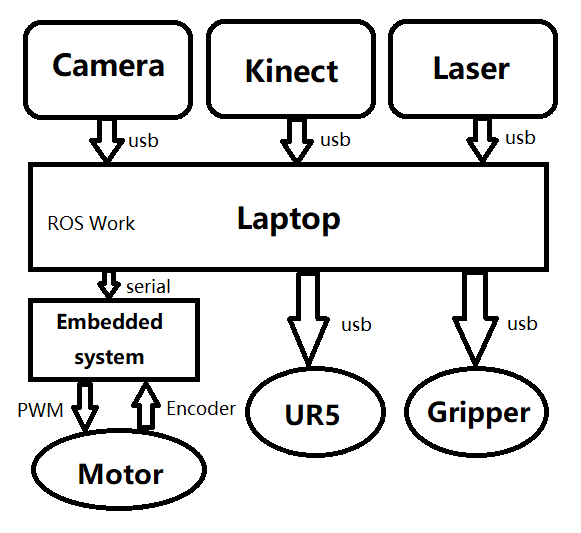
\includegraphics[scale=0.5]{commuication_arch.png}
    \caption{The architecture of the hardware-communication layer}
    \label{arch_comm}
\end{figure}

\subsubsection{The logic layer}
\ 

Most important robot functions are implemented in this layer. The main components in this layer include:
\begin{enumerate}
    \item Navigation: Mapping, localization, route-planning and collision avoidance
    \item Vision: Human recognition, object recognition and their tracking.
    \item Speech: Speech recognition and synthesis
    \item Move it: Manipulation with feedback from vision and laser
\end{enumerate}

\subsubsection{The decision layer}
\ 

Task planning is done in decision layer. For different tasks, modules in decision layer run as state machine. They integrate different information from the low layer to judge the state they are in and then give different orders or make different responses. Each module deal with a single task, sharing the common information from the lower layers.



\section{Mechanical Design}
To complete mostt of home serving tasks, our robot consists of three major parts: chassis based on Mecanum wheel, Ball screw Actuator and robot arm including hand. Tinker is about 150cm in height. 
\subsubsection{Chassis}
Tinker can move in any direction easily owing to the Mecanum chassis. The chassis consists of 4 separated Mecanum wheel systems, each of which consists of a Mecanum wheel, a brushless DC motor (50W24V), a worm gear box and a brush-less DC motor driver. The PC sends control message to the ZYNQ to command the chassis to move as planed based on ROS. The chassis has a size of $800\text{mm} \times 500\text{mm}\times 200\text{mm}$.
\begin{figure}[!t]
\centering
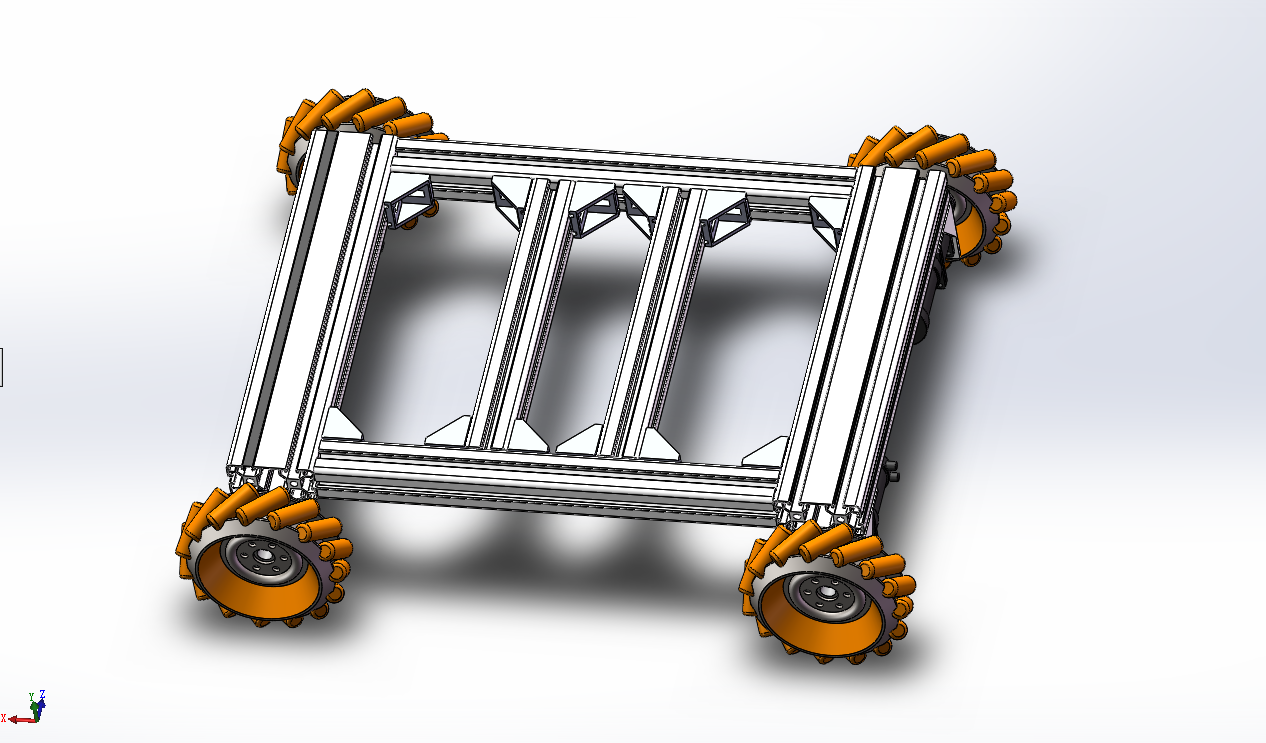
\includegraphics[scale=0.5]{base.jpg}
    \caption{Chassis}
\end{figure}

\subsubsection{Robot arm and hand}
The robot arm is the most major part of the mobile robot, used to grasp objects. The complete arm consists of a 3-axis cascade robot arm and a 2-axis robot hand. The 3-axis arm consists of 2 bent joints and a rotate joint; the 2-axis hand consists of a rotate joint which controls the posture and a joint which achieves grasping objects. We use 24V geared DC motor for the arm and MX-64R (Robotis series) as the steering engines for the hand. The maximum length of the arm is about 800mm and it can grasp a 1000g object at maximum length, which is enough in most situations. 
\begin{figure*}[!t]
	\centering
    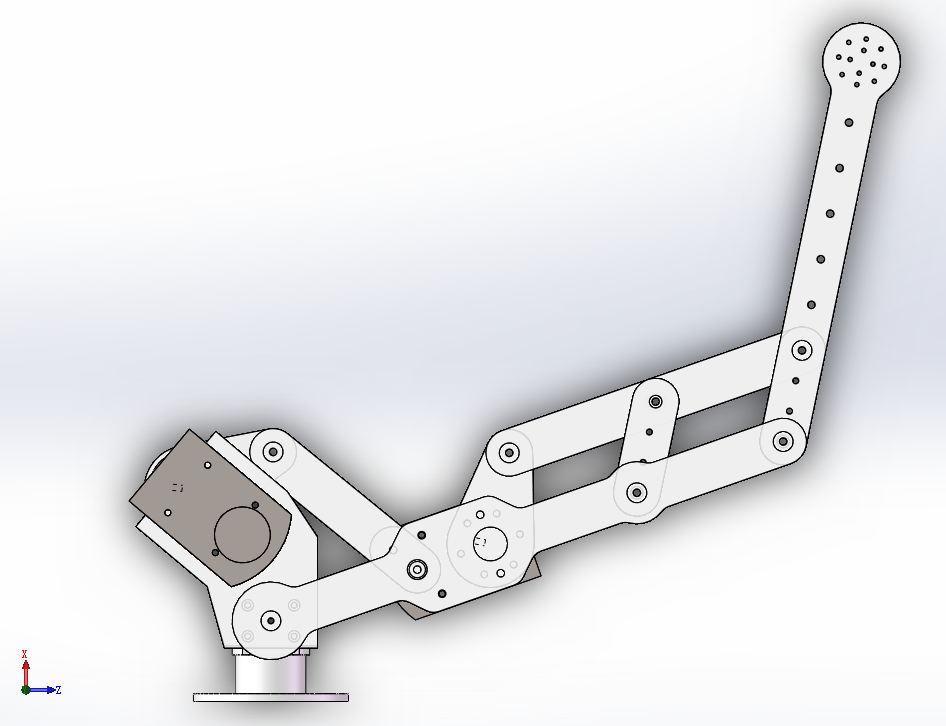
\includegraphics[scale=0.5]{arm.jpg}
    \caption{Robotic Arm}
\end{figure*}

\subsubsection{Ball screw Actuator}
The bottom of the robot arm is fixed on the Ball screw Actuator so that the arm can be raised or lowered freely, quickly and smoothly. The lift platform enables the robot to manipulate objects of various height. Besides, it provides more workspace.




\section{Software Engineering}
\subsection{Computer Vision}
Computer vision is indispensable for tinker to accomplish multiple tasks including person recognition, object manipulation and environment modeling.
\subsubsection{Human Tracking}
For human tracking and following, we implemented the TLD (Track-Learning-Detection) algorithm\cite{kalal2012tracking}. TLD was proposed by Zdenek Kalal and is currently the state-of-art real time tracking algorithm. It combine the traditional tracking and detection algorithm so that it is more robust in consideration of distortion and partial occlusions. TLD algorithm consists of three modules as its name indicated. Tracking module estimate moving direction of the object according to the difference between two adjacent frames. Detection module detect the object in each frame independently. Learning module integrate the results of the tracking module and detection module to correct the detection errors and update the features of the target object.
We applied the TLD algorithm to human tracking and following tasks. Before the robot starts following, the human partner to be followed will be asked to stand in front of Kinect and the robot will record his/her features. When the instructor starts moving around, the robot will track and keep up with him. The robot also uses the depth information to keep away from the instructor at a safe distance.
\subsubsection{Face Recognition}
For human-robot interaction, a robot is required to recognize different masters or guests in home service. We developed a face recognition system with two process: enrollment and recognition. During the enrollment process, a man is asked to stand in front of the RGB camera. A face detector based on haar feature from OpenCV is applied and the detected face will be stored. For a single person, the system stores 3-5 pictures.
We implemented the face recognition algorithm based on sparse representation \cite{wright2009robust}. A redundant dictionary is trained offline using a set of training faces. The algorithm seeks the most sparse representation coefficient by solving a L1 optimization problem. The residual errors for different classes (persons) tell who is the unknown person: if the residual error for a specific class, for example, person A, is smaller than a specified threshold and the errors for other classes are larger than another specified threshold, the newcoming person is identified as person A. More details of the face recognition pipeline can be found in \cite{xia2015human}.
%\begin{figure}[!t]
%	\centering
%    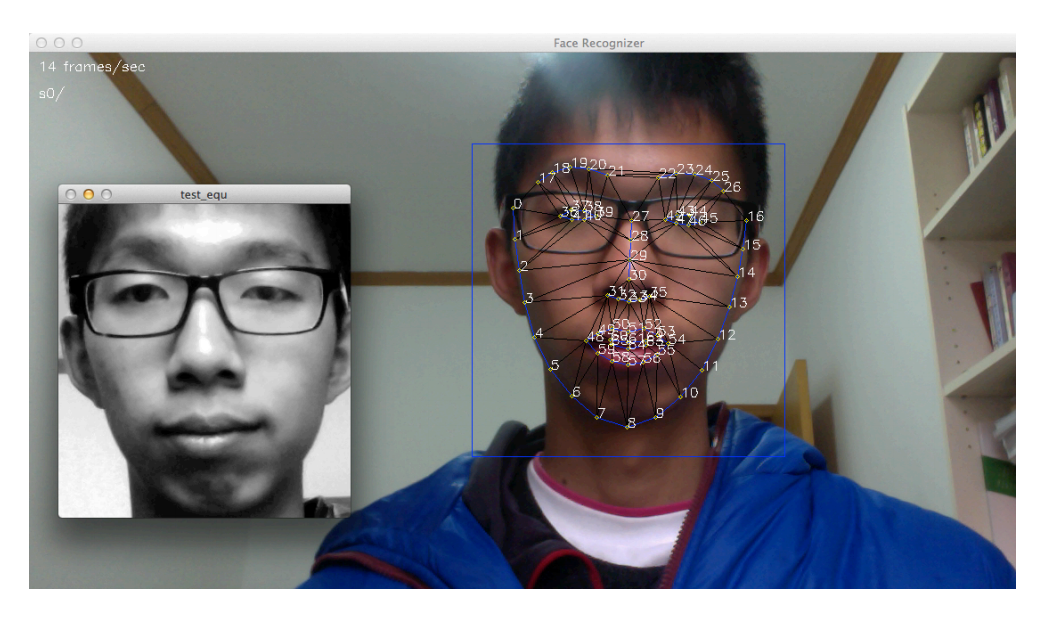
\includegraphics[scale=0.5]{face.png}
%    \caption{face recognition}
%\end{figure}
\subsubsection{Object recoginition and manipulation}
Tinker uses a two-phase approach to recognize objects and precisely manipulate them. In the first phase, a point cloud is built from the Kinect depth camera. Hough transform and an entropy-based filter is applied to the point cloud to remove the backgroud. Then a euclidean clustering will give the region of interest. A typical image of the filtered point cloud is given below:
\begin{figure}[!t]
	\centering
    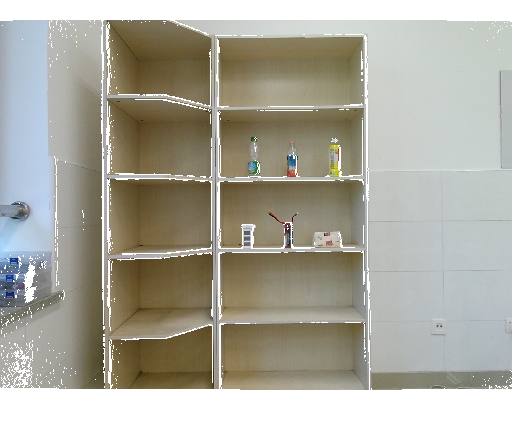
\includegraphics[scale=0.5]{original.png}
    \caption{Original image.}
\end{figure}

\begin{figure}[!t]
	\centering
    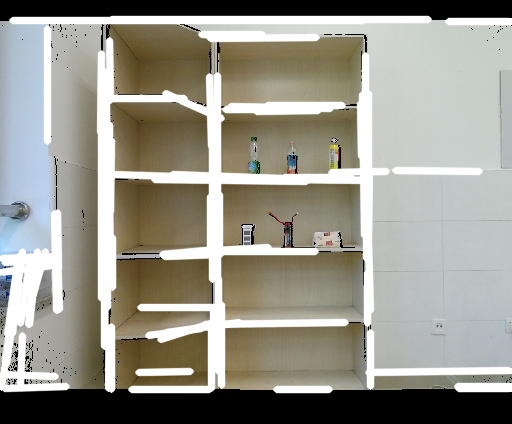
\includegraphics[scale=0.5]{filtered.png}
    \caption{Filtered image.}
\end{figure}

In the second phase, the approximate location of object is given to the robot arm controller, another usb camera placed in the hand of the robot arm will guide the arm to precisely manipulate the object. First, the hand is moved to directly face the location of the region of interest at about 40 cm away. A similar image processing pipeline is used to find the object in the image given by the camera in hand. After getting the image of the object, it is matched with the pre-captured image set by convolution the image with the templates to find the best mattch. Precision of the location found in this phase is significantly improved due to a much closer camera place. Then the robot arm will be guided by the camera using a feedback procedure to place the object in the middle of the camera image. Thus, the chance of missing the object is reduced.

\begin{figure}[!t]
	\centering
    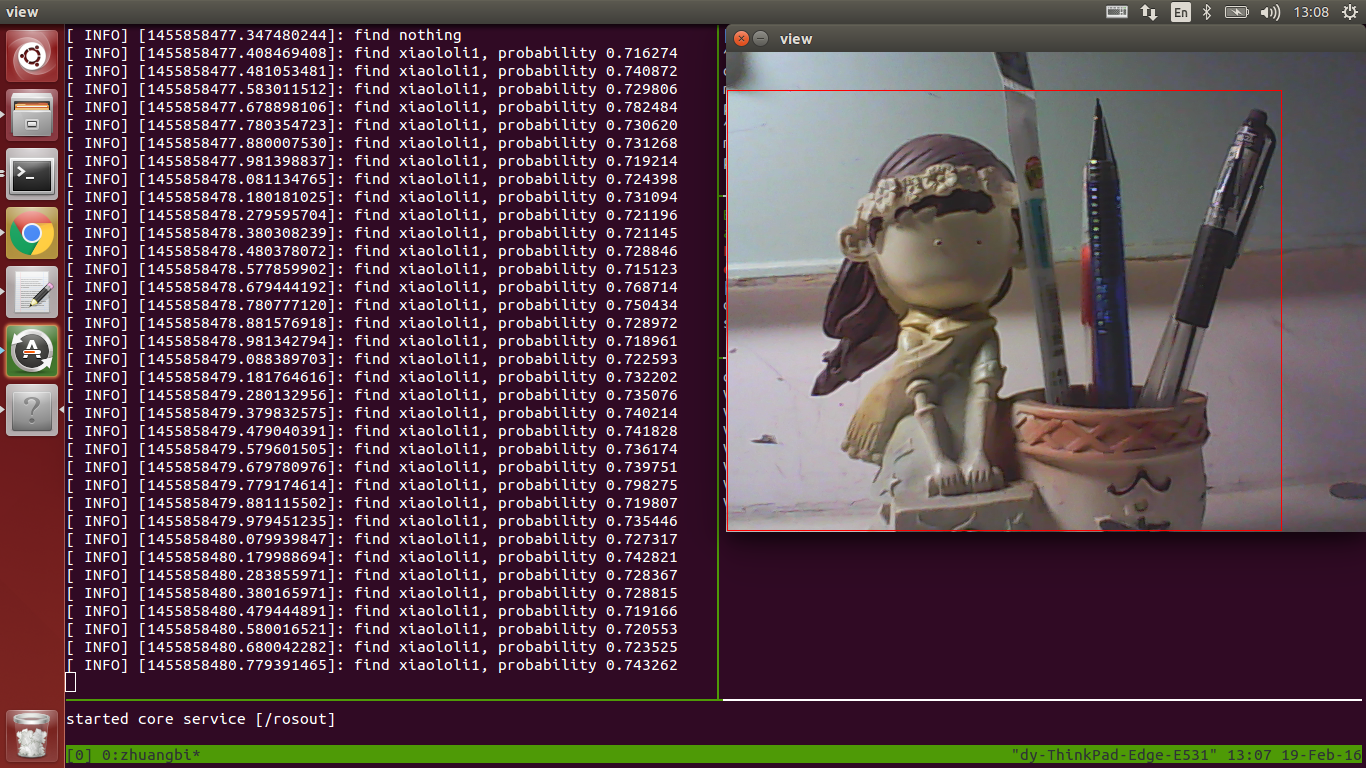
\includegraphics[scale=0.3]{object_found.jpg}
    \caption{Objects found from the camera}
\end{figure}


\subsection{Navigation}
\subsubsection{Simultaneous Localization and Mapping}
SLAM is one of the most important algorithms for a mobile autonomous robot, which enables a robot to navigate and explore in an unknown environment \cite{grisetti2007improved}. Mapping requires the robot to record, integrate and update the former information it have got about the surroundings while Localization requires the robot to know the location of itself refer to the estimated environment. Using a laser range finders (LRFs), we adopted the SLAM package to estimate the location and its surroundings in the form of 2D occupancy grid map. The raw data from LRFs are collected as the input of the algorithm. Features, or landmarks are then extracted from the environment. When the robot moves around, these features are used to estimate where it moves. It is called Laser-Scan-Matcher process. However, the estimation of this process is imprecise and the error accumulates. The GMapping process is adopted, using an EKF (Extended Kalman Filter) to correct the estimated result. Based on the final map generated, the robot plans its path and explores the unknown environment.
We also implemented SLAM using color and depth camera, also called vSLAM \cite{se2005vision}, so that a 3D map can be obtained, which is more precise in complicated environment. Building map using vSLAM is still a experimental feature for tinker and needs further refining.
\subsubsection{Navigation}
Navigation is one of the basic function that a mobile autonomous robot must have. The robot needs to plan the route from its current position to the goal. An A* algorithm is used to find the route considering both distance and  collision avoidance. Moreover, the robot must be able to handle unexpected obstacles when moving around. The navigation package is applied and modified for the tinker robot. Parameters in the move\_base package are tuned and the navigation task can be achieved functionally but the behavior and speed is far from satisfactory. We extended a local  which subscribes the origin global plan and linearizes the curve. In this way, the whole processing could be more fluently. 
To avoid small objects and non cylinder-like objects like chairs and cups on the floor, we use depth cameras including a kinect2 and a primesense to build another local obstacle layer. Since pointcloud tend to be noisy, we filter this obstacle layer to achieve more stable navigation performance.
This year, a new social layer was added to classify Bayesian data. When a person enters the camera line of sight, he will be judged to be living and marked. Even if he leaves the camera line of sight, he will be tagged in the clustering model formed by radar to provide better effect for obstacle avoidance. 

\begin{figure*}[!t]
	\centering
	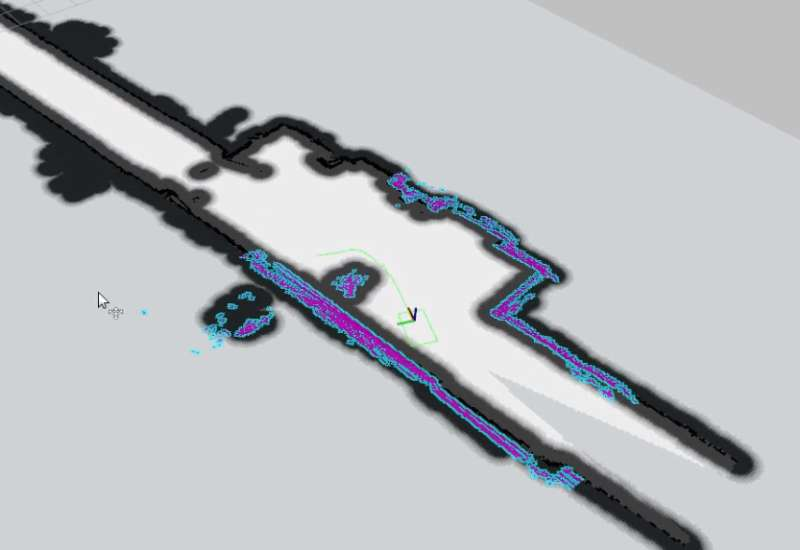
\includegraphics[scale=0.4]{niv.jpg}
	\caption{Navigation show}
\end{figure*}


\subsection{Speech Recognition}
For 2019 competition, we implement speech interaction system based on google TTS(Text-To-Speech) and STT(Speech-To-Text) Cloud API. To overcome communication delay from robot and cloud platform, we realize a stream based audio transfrom method for speech recognition. Moreover, Tinker caches a huge amount of audio response template locally to accelerate robot correspondance.

After speech to text layer, dialogue system consists of a simple keyword parser, which takes keywords in certain patterns to operate task switches: When the software recognizes a sequence with one of the predefined patterns, the robot interprets one's intention and makes corresponding responses. Sound source localization method is realized by IFLYTEK develop toolkit.




\section{Team repository}
Our team repository can be found at \url{https://github.com/tinkerfuroc}. The repository may be of help to other teams by providing:
\begin{enumerate}
    \item Implementation of all the algorithms and needed parameters described in the paper
    \item Robot setup scripts and tools
    \item Code for RoboCup@Home tasks 
\end{enumerate}

\section{3rd Party Dependencies}
\begin{enumerate}
    \item \href{www.ros.org}{ROS}
    \item \href{github.com/ros-planning/navigation}{ROS Navigation Stack}
    \item \href{github.com/code-iai/iai\_kinect2}{iai\_kinect2}
    \item \href{github.com/pjreddie/darknet}{darknet(tensorflow fast yolo)}
    \item \href{www.tensorflow.org}{tensorflow}
    \item \href{www.faceplusplus.com}{face++}
\end{enumerate}


%As Tinker is young, there are still a lot of things to learn and improve.

%Citation test \cite{xia2015human}.

\section*{Acknowledgement}
The authors of this paper would like to thank previous team members of Tinker@Home 2014, Tinker@Home2015, Tinker@Home2017 for their help and support through out building the robot and writing this manuscript. The authors would also like to thank Google, IFLYTEK, Questyle Audio, and Mech-Mind, for their material or technology support. 


\bibliography{main.bib}
\bibliographystyle{IEEEtran}


\end{document}
